\documentclass{article}
\usepackage[utf8]{inputenc}
\usepackage[spanish,mexico]{babel}
\usepackage[margin=2.3cm]{geometry}
\usepackage{graphicx}
\usepackage[export]{adjustbox}
\usepackage{caption}
\usepackage{subcaption}
\usepackage{fancyhdr}
\usepackage{lipsum}
\usepackage{float}
\usepackage{enumerate}
\usepackage{array}
\usepackage{float}

% >
\usepackage{ tipa }

%\usepackage{multirow}
\usepackage[spanish,es-tabla]{babel}

% Comentario en varias líneas
\usepackage{comment}

% Importar código de algún lenguaje
%\usepackage{listings}
%\lstset{
%  language=Scheme
%}
\usepackage{xcolor}

\definecolor{codegreen}{rgb}{0,0.6,0}
\definecolor{codegray}{rgb}{0.5,0.5,0.5}
\definecolor{codepurple}{rgb}{0.58,0,0.82}
\definecolor{backcolour}{rgb}{0.95,0.95,0.92}

%\lstdefinestyle{mystyle}{
%    backgroundcolor=\color{backcolour},
%    commentstyle=\color{codegreen},
%    keywordstyle=\color{magenta},
%    numberstyle=\tiny\color{codegray},
%    stringstyle=\color{codepurple},
%    basicstyle=\ttfamily\footnotesize,
%    breakatwhitespace=false,
%    breaklines=true,
%    captionpos=b,
%    keepspaces=true,
%    numbers=left,
%    numbersep=5pt,
%    showspaces=false,
%    showstringspaces=false,
%    showtabs=false,
%    tabsize=2
%}

%\lstset{style=mystyle}

% Evitar sangrías
\setlength{\parindent}{0cm}

% Formato para estructuras como with.
\usepackage{listings}

% Código
\newcommand{\code}[1]{\textcolor{white!25!black}{\texttt{#1}}}

% Letter colors.
\usepackage{xcolor}

% Columnas multiples
\usepackage{multicol}

\usepackage{amsmath}
%%\usepackage{graphicx}
%%\usepackage{subcaption}
\usepackage{amsmath}
\usepackage{amssymb}
\usepackage{amsthm}
\usepackage{url}

%%Tablas con color
\usepackage{xcolor, colortbl}
\usepackage{array, multirow, multicol}
\cellcolor[modelo color]{color}

\pagestyle{fancy}
\fancyhf{}

\title{Facultad de Ciencias, UNAM}
\date{\today}

\begin{document}

\thispagestyle{empty}

	\begin{figure}[ht]
	   \minipage{0.76\textwidth}
			
\includegraphics[width=4cm]{Logo_UNAM.png}
			\label{EscudoUNAM}
	   \endminipage
	   \minipage{0.32\textwidth}
			
\includegraphics[height = 4.9cm ,width=4cm]{Logo_FC.png}
			\label{EscudoFC}
		\endminipage
	\end{figure}

	\begin{center}
	\vspace{0.8cm}
	\LARGE
	UNIVERSIDAD NACIONAL AUTÓNOMA DE MÉXICO

	\vspace{0.7cm}
	\LARGE
	FACULTAD DE CIENCIAS

	\vspace{0.8 cm}
	\Large
	\textbf{Resumen}

	\vspace{0.8 cm}
	\normalsize
	INTEGRANTES \\
	\vspace{.2cm}
	\large
	\textbf{Torres Valencia Kevin Jair - \texttt{318331818}}\\
        \textbf{Aguilera Moreno Adrián - \texttt{421005200}}\\
        \textbf{Natalia Abigail Pérez Romero  - \texttt{31814426}}\\
	%\textbf{Nombre - \texttt{Número de cuenta}}

	\vspace{1 cm}
	\normalsize
	PROFESOR \\
	\vspace{.2cm}
	\large
	\textbf{Miguel Ángel Piña Avelino}

	\vspace{1 cm}
	AYUDANTE \\
	\vspace{.2cm}
	\large
	\textbf{Pablo Gerardo González López}
	\vspace{1.3cm}

	\normalsize
	ASIGNATURA \\
	\vspace{.2cm}
	\large
	\textbf{Computación Distribuida}

	\vspace{1 cm}
	\today
	\end{center}

	\newpage
	Nuestra exposición comienza con una breve introducción sobre definición y
propiedades de los relojes vectoriales. Posteriormente damos presentación
a las aplicaciones sobre estos. Tenemos las siguientes aplicaciones:
\begin{itemize} 
%%%%%%%%%%%%%%%%%%%%%%%%%%%%%%%%%%%%        Dynamo
\item [$\blacktriangleright$]{\bf El caso DynamoDB}\\

De manera general lo utilizan para poder controlar el orden de los registros
de multiversión. Amazon utilizó los relojes vectoriales con reconciliación 
durante las lecturas para resolver el problema de alta disponibilidad para 
escrituras, permitiendoles tener una ventaja de que el tamaño de la versión 
está desvinculado de las tasas de actualización. Un reloj vectorial es 
efectivamente una lista de pares (nodo, contador). Y este estará asociado 
con cada versión de cada objeto.

\begin{itemize}
\item {\bf ¿Para que los utiliza?}\\
Para capturar la causalidad entre diferentes versiones del mismo objeto.
DynamoDB nos permitirá determinar si dos versiones de un objeto están en ramas 
paralelas o tienen un orden causal, examinando sus relojes vectoriales.

Si los contadores del reloj del primer objeto son menores o iguales que todos
los nodos del segundo reloj, entonces el primero es un ancestro del segundo y
puede olvidarse. De lo contrario, se considera que los dos cambios están en
conflicto y requieren reconciliación.

\item {\bf ¿Como lo hace}\\
Cuando un cliente desea actualizar un objeto, debe especificar qué versión está
actualizando. Esto se hace pasando el contexto que obtuvo de una operación de
lectura anterior, que contiene la información del reloj vectorial.\\

\begin{center}
    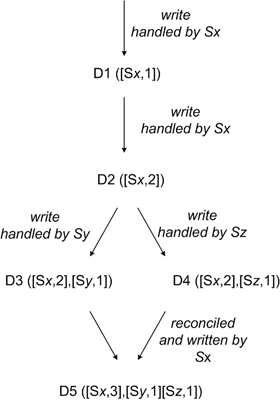
\includegraphics[scale=0.5]{Imagenes/D1.png}
    \end{center}

Al procesar una solicitud de lectura, si Dynamo tiene acceso a varias ramas que
no se pueden reconciliar sintácticamente, devolverá todos los objetos en las
hojas, con la información de versión correspondiente en el contexto. Se considera
que una actualización que usa este contexto ha reconciliado las versiones
divergentes y las ramas se contraen en una sola versión nueva.

\item {\bf Una posible desventaja}\\
Es que el tamaño de los relojes vectoriales puede crecer si muchos servidores
coordinan las escrituras en un objeto. En caso de particiones de red o fallas 
de múltiples servidores, las solicitudes de escritura pueden ser manejadas por 
nodos que no están en los primeros N nodos en la lista de preferencias. Este 
problema no ha surgido en la producción y, por lo tanto, este problema no se ha
investigado a fondo por parte de amazon. Para evitar lo anterior implementa un
esquema de truncamiento de reloj: Junto con cada par (nodo, contador), Dynamo 
almacena una marca de tiempo que indica la última vez que el nodo actualizó 
el elemento de datos. Cuando el número de pares en el reloj vectorial alcanza 
un umbral, el par más antiguo se elimina del reloj.
\end{itemize}
%%%%%%%%%%%%%%%%%%%%%%%%%%%%%%%%%%%%        Relojes Vectoriales dinámicos
\item [$\blacktriangleright$] {\bf Relojes Vectoriales dinámicos}\\

A menudo el número de procesos participando en un computo distribuido no es constante, 
por lo que los relojes debe ser capaces de crecer. El tamaño del vector está limitado 
por dos veces el número de procesos de los que el proceso de mantenimiento ha recibido 
(directa o indirectamente) valores de reloj. Cada proceso $p_i$ mantiene su propio reloj 
lógico $C_i$ el cual es una matriz de dos columnas, variable en su número de filas, 
donde $C_i(e_i^x)[k,2]$, en $e_i$ almacena el valor del último reloj vectorial conocido 
por $p_i$ del proceso cuyo ID está en $C_i(e_i^x)[k,1]$.\\


\begin{center}
    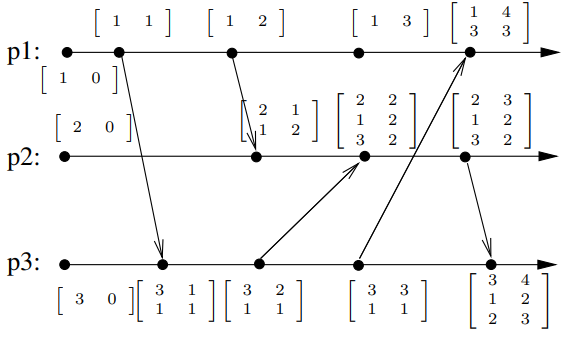
\includegraphics[scale=0.6]{Imagenes/rvd01.png}
    \end{center}

Inicialmente, el reloj consiste de una sola fila con $C_i(e_i^0)[1,1]=i$ y $C_i(e_i^0)[1,2]=0$.
Las reglas para actualizar son las siguientes:
\begin{itemize}
\item Al recibir el $m$ de $e_i^x$, entonces $\forall l$ que no exceda el número de filas 
en \\
$C_j(e_j^y)$: $C_j(e_j^y) = max\{C_i(e_i^{x-1})[k,2], C_j(e_j^y)[1,2]\}$, donde $C_j(e_j^y)$ 
la matriz de reloj del evento enviado en el proceso $J$ que envió $m$ al proceso $i$, 
y $C_j(e_j^y)[l,1]=C_i(e_i^x)[k,1]$

\item Si no existe $k$ tal que $C_i(e_i^x)[k,1] = C_j(e_j^y)[l,1]$ para cualquier l, 
entonces una nueva fila es añadida a \\
$C_i(e_i^x)$ con $C_i(e_i^x)[k,1] = C_j(e_j^y)[l,1]$ y $C_i(e_i^x)[k,2] = C_j(e_j^y)[l,2]$

\item Si $e_i^x$ es cualquier evento, entonces el proceso incrementa su reloj vectorial: 
$C_i(e_i^x)[1,2] = C_i(e_i^{x-1})[1,2]+1$
\end{itemize}



%%%%%%%%%%%%%%%%%%%%%%%%%%%%%%%%%%%%        Determinando Propiedades globales
\item  [$\blacktriangleright$] {\bf Determinando Propiedades globales}\\

Evento relevante: En algún nivel de abstracción, sólo un subconjunto de los eventos 
son relevantes. Por ejemplo, en algunas aplicaciones sólo la modificación de algunas 
variables locales, o el procesamiento de ciertos mensajes específicos son relevantes. 
Dado un computo distribuido $\widehat{H}=(H,\xrightarrow[]{ev})$, sea $R\subset H$ 
los eventos relevantes.\\

{\bf Definición}. Relación causal de Precedencia, denotada como $\xrightarrow[]{re}$:
$$\forall e_1,e_2 \in R : (e_1 \xrightarrow[]{re} e_2) \iff (e_2 \xrightarrow[]{ev} e_1)$$
Esta relación es la proyección de $\xrightarrow[]{ev}$ sobre los elementos de R.
Sean $e_1,e_2 \in R$. Si $e_1$ es \textbf{predecesor inmediato de} $e_2$ entonces:
$$(e_1 \xrightarrow[]{re} e_2) \wedge (\nexists e \in : (e_1 \xrightarrow[]{re} e) \wedge (e \xrightarrow[]{re}e_2))$$

\begin{center}
    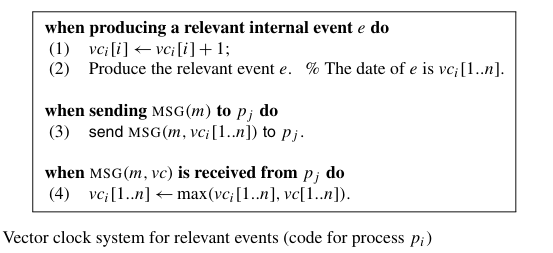
\includegraphics[scale=0.7]{Imagenes/eventosRelevantes02.png}
    \end{center}
\begin{center}
    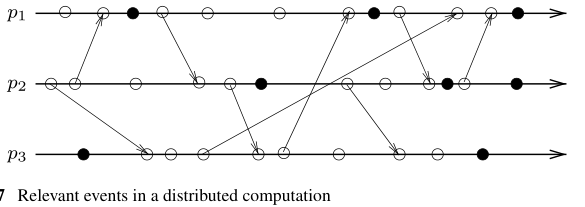
\includegraphics[scale=0.6]{Imagenes/eventosRelevantes01.png}
    \end{center}

$\bullet$ El problema del seguimiento del predecesor inmediato 
(Immediate predecessor tracking IPT).\\
Consiste en asociar a cada evento relevante el conjunto de eventos relevantes que son 
sus predecesores inmediatos. Además, esto se ha hecho sobre la marcha y sin añadir 
mensajes de control. La determinación de los predecesores inmediatos consiste en 
calcular la reducción transitiva (o diagrama de Hasse) del orden parcial 
$\widehat{R}=(R,\xrightarrow[]{re})$.
%%%%%%%%%%%%%%%%%%%%%%%%            algoritmo ipt04 ---------Imagenes
\begin{center}
    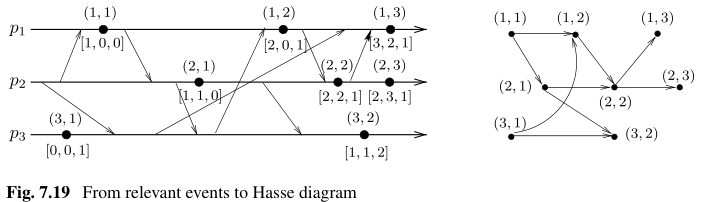
\includegraphics[scale=0.6]{Imagenes/eventosRelevantes03.png}
    \end{center}
%%%%%%%%%%%%%%%%%%%%%%%%%%%%%%%%%%%%        Detección de una conjunción de predicados locales estables
\item [$\blacktriangleright$] {\bf Detección de una conjunción de predicados}

\begin{itemize}
\item {\bf Def.} Un predicado es local para $p_i$ \textit{\textbf{Sii}} se 
encuentra en variables de $p_i$ solamente.

\item {\bf Def.} El predicado $LP_i$ es estable \textit{\textbf{Sii}} en 
cuanto se vuelva verdadero, este permanece así siempre.

\item {\bf Notación} $\sigma_i \models LP_i$. Indica que el estado local 
$\sigma_i$ de $p_i$ satisface el predicado $LP_i$.

\item {\bf Def.} Sea $\{p_1, \dotsm, p_n\}$ un sistema distribuido y 
$LP_1, \dotsm, LP_n$ $n$ predicados locales, uno por proceso (con su 
respectivo proceso). Un \textit{estado global consistente} 
$\sum = (\sigma_1, \dotsm, \sigma_n)$ satisface el predicado global
$LP_1 \land \dotsm \land LP_n$ denotado por 
\[\sum \models \bigwedge_i LP_i\]
siempre que $\bigwedge_i (\sigma_i \models LP_i)$.

\item {\bf Problema:} Detectemos sobre la \textit{historia} del sistema, y 
sin utilizar controles de mensajes adicionales, el primer estado global 
consistente $\Sigma$ que satisface una conjunción de predicados locales estables.
\end{itemize}
%%%%%%%%%%      ConjunctionSatableLocalPredicates01 --------Imagenes

%%%%%%%%%%%%%%%%%%%%%%%%%%%%%%%%%%%%        Un problema de conjuntos: Conjuntos Posibles e Imposibles
\item {\bf Un problema de conjuntos: Conjuntos Posibles e Imposibles}\\

El problema de los \textit{conjuntos imposibles} establece:\\
{\bf Dado un conjunto con n etiquetas vectoriales de k entradas cada una, 
decidir si es posible o no.}\\
%%%%%%%%%%  Imagenes ProblemaConjuntos01 ------> Imagen
{\bf Ejemplo:}
\begin{center}
    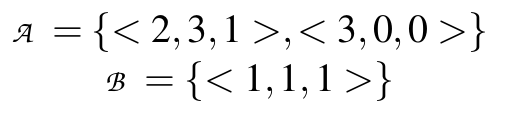
\includegraphics[scale=0.2]{Imagenes/Conjuntos.png}
    \end{center}
\begin{center}
    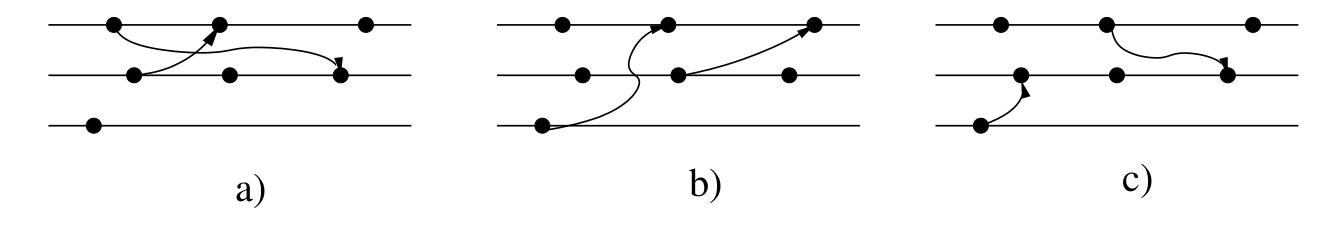
\includegraphics[scale=0.25]{Imagenes/Historia.png}
    \end{center}

\end{itemize}
        \newpage\section*{Referencias}
\begin{itemize}
\item Michel Raynal. Distributed Algorithms for Message-Passing Systems. Springer, 2013.
\item Amazon's Dynamo (n. d.). Allthingsdistributed. Consultado en diciembre 12, 2022, de \\
https://www.allthingsdistributed.com/2007/10/amazons\_dynamo.html
\end{itemize}
\end{document}